\phantomsection

\chapter{\uppercase{HIERARCHICAL FUSION FOR MULTIMODAL DIALOG ACT CLASSIFICATION}}

\section{Label Distribution for MRDA and EMOTyDA}
\label{sec:label_distribution}

\autoref{fig:label_distribution} shows the label distribution for the MRDA and EMOTyDA datasets.
\begin{figure*}[ht]
  \centering
  \begin{minipage}{0.48\textwidth}
    \centering
    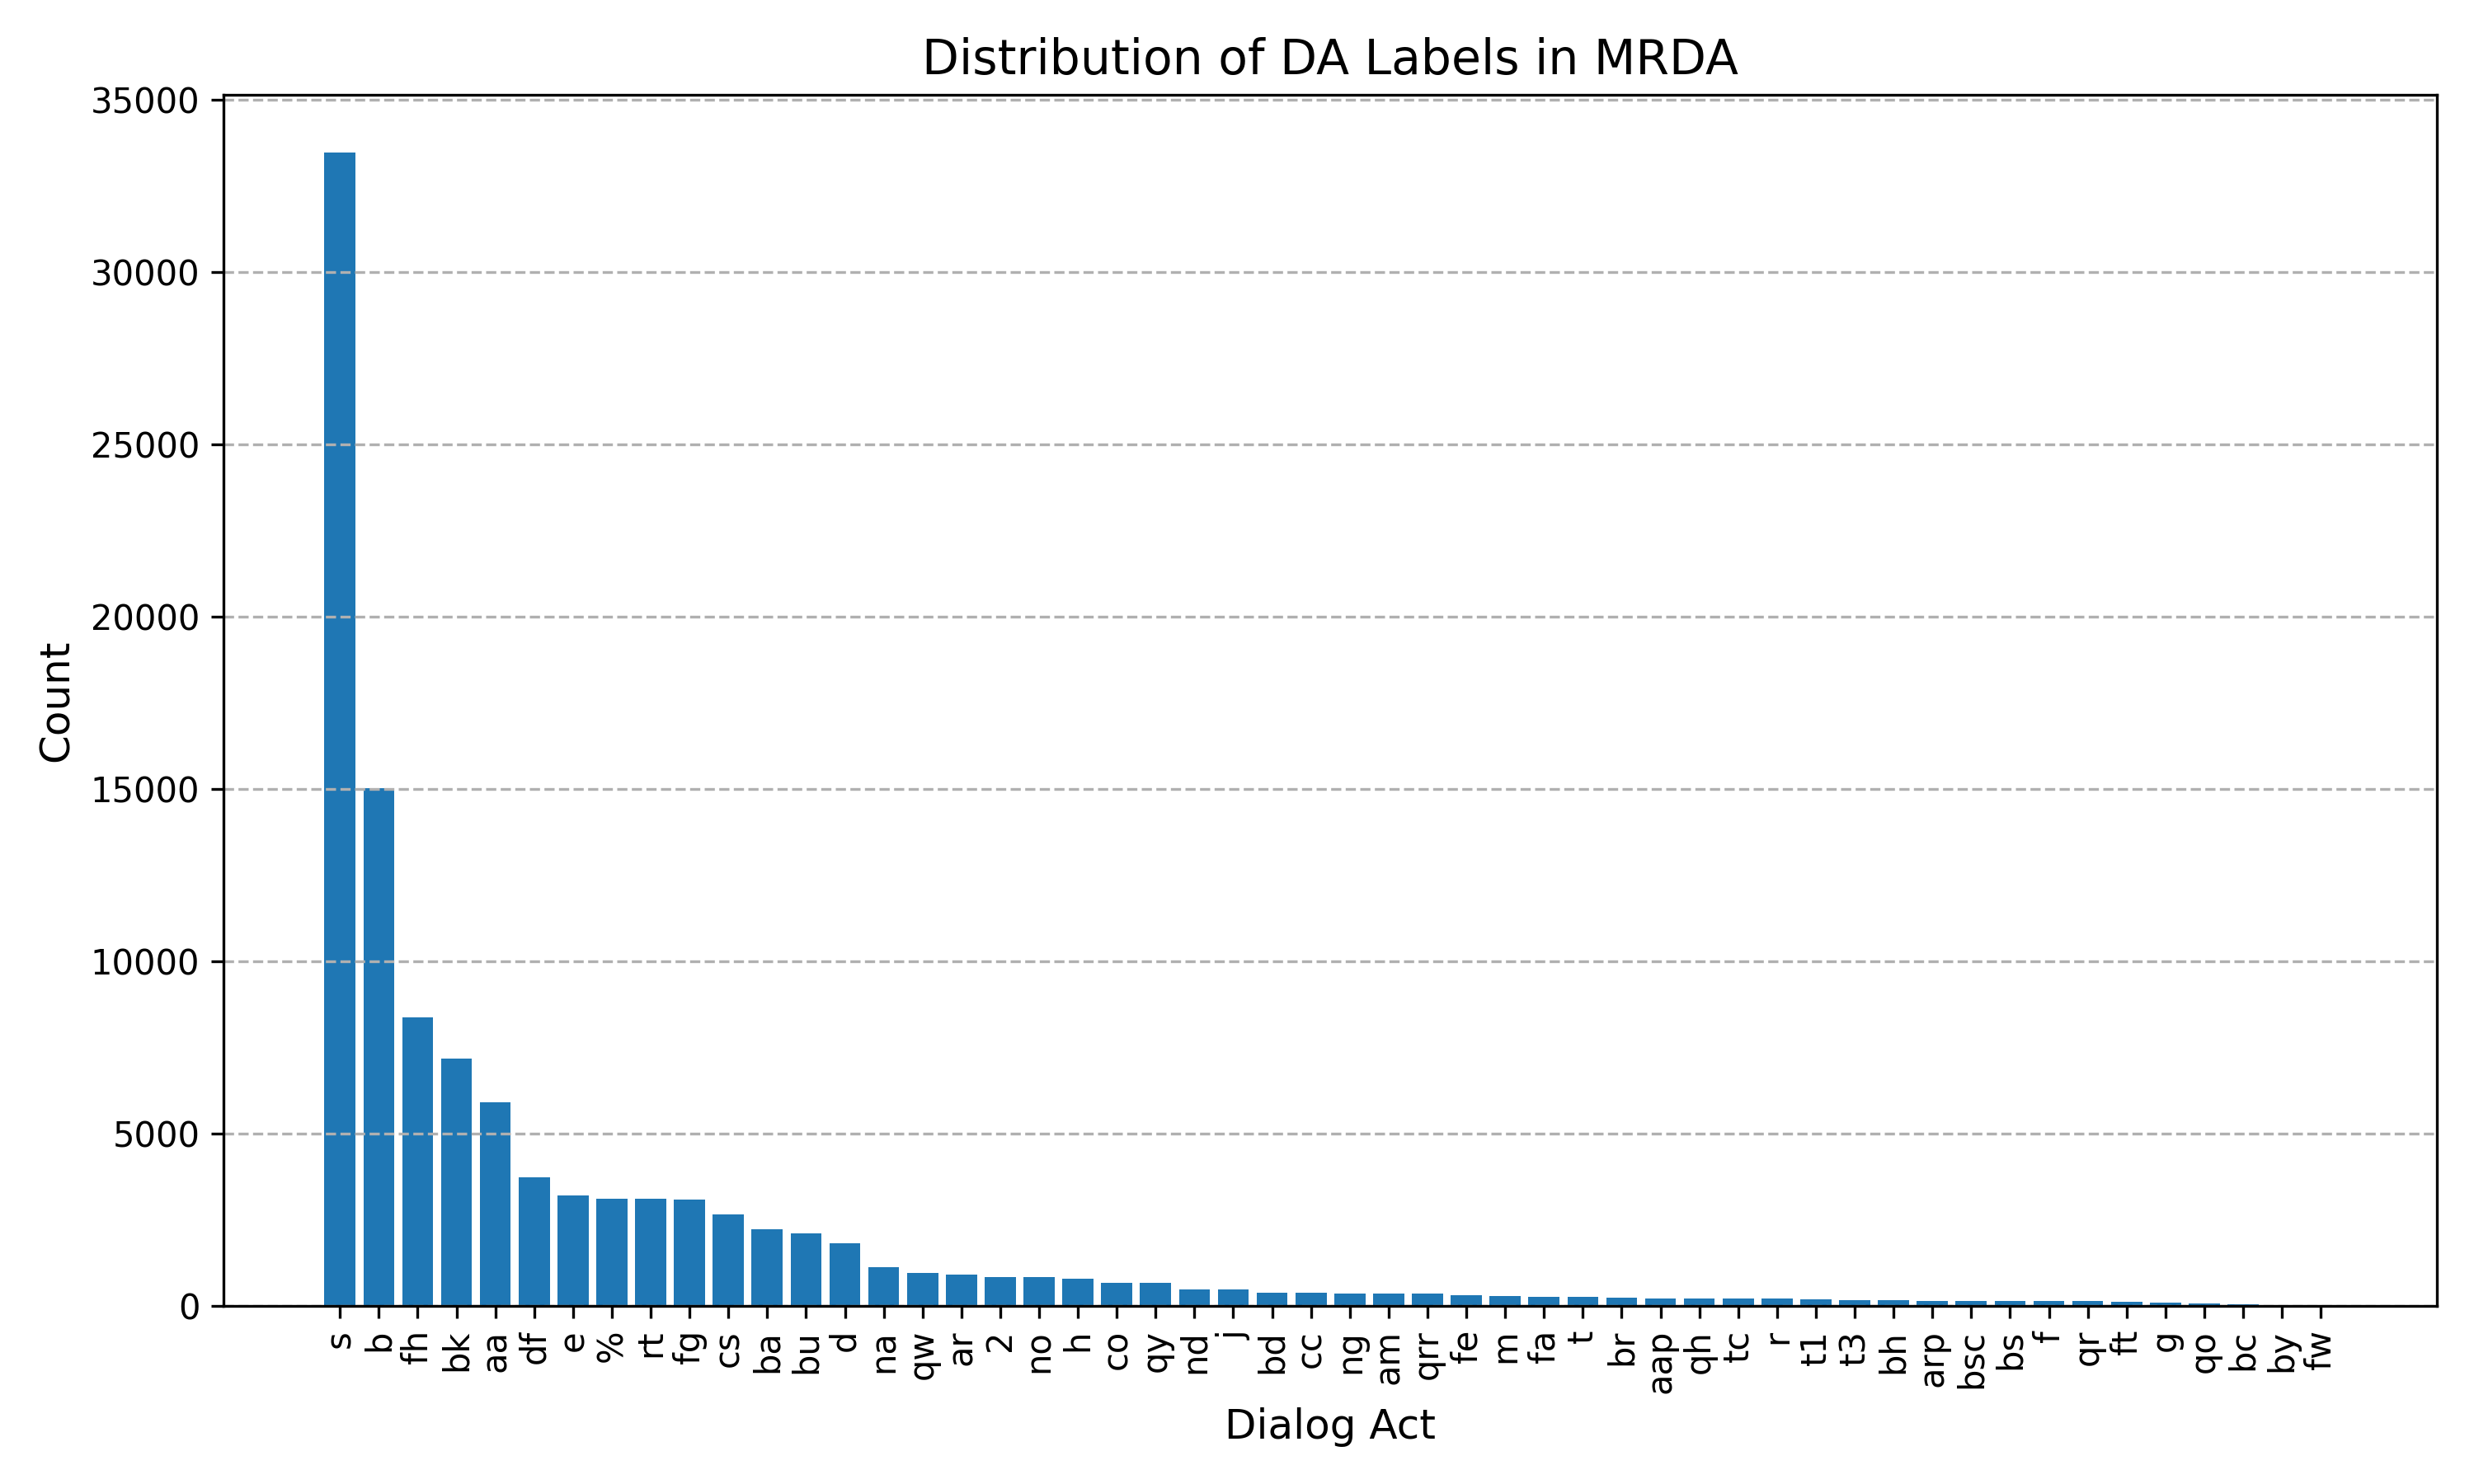
\includegraphics[width=\textwidth, scale = 5]{images/da_tag3_counts_mrda.png}
    \caption*{(a) MRDA}
    \label{fig:image1}
  \end{minipage}
  \hfill
  \begin{minipage}{0.48\textwidth}
    \centering
    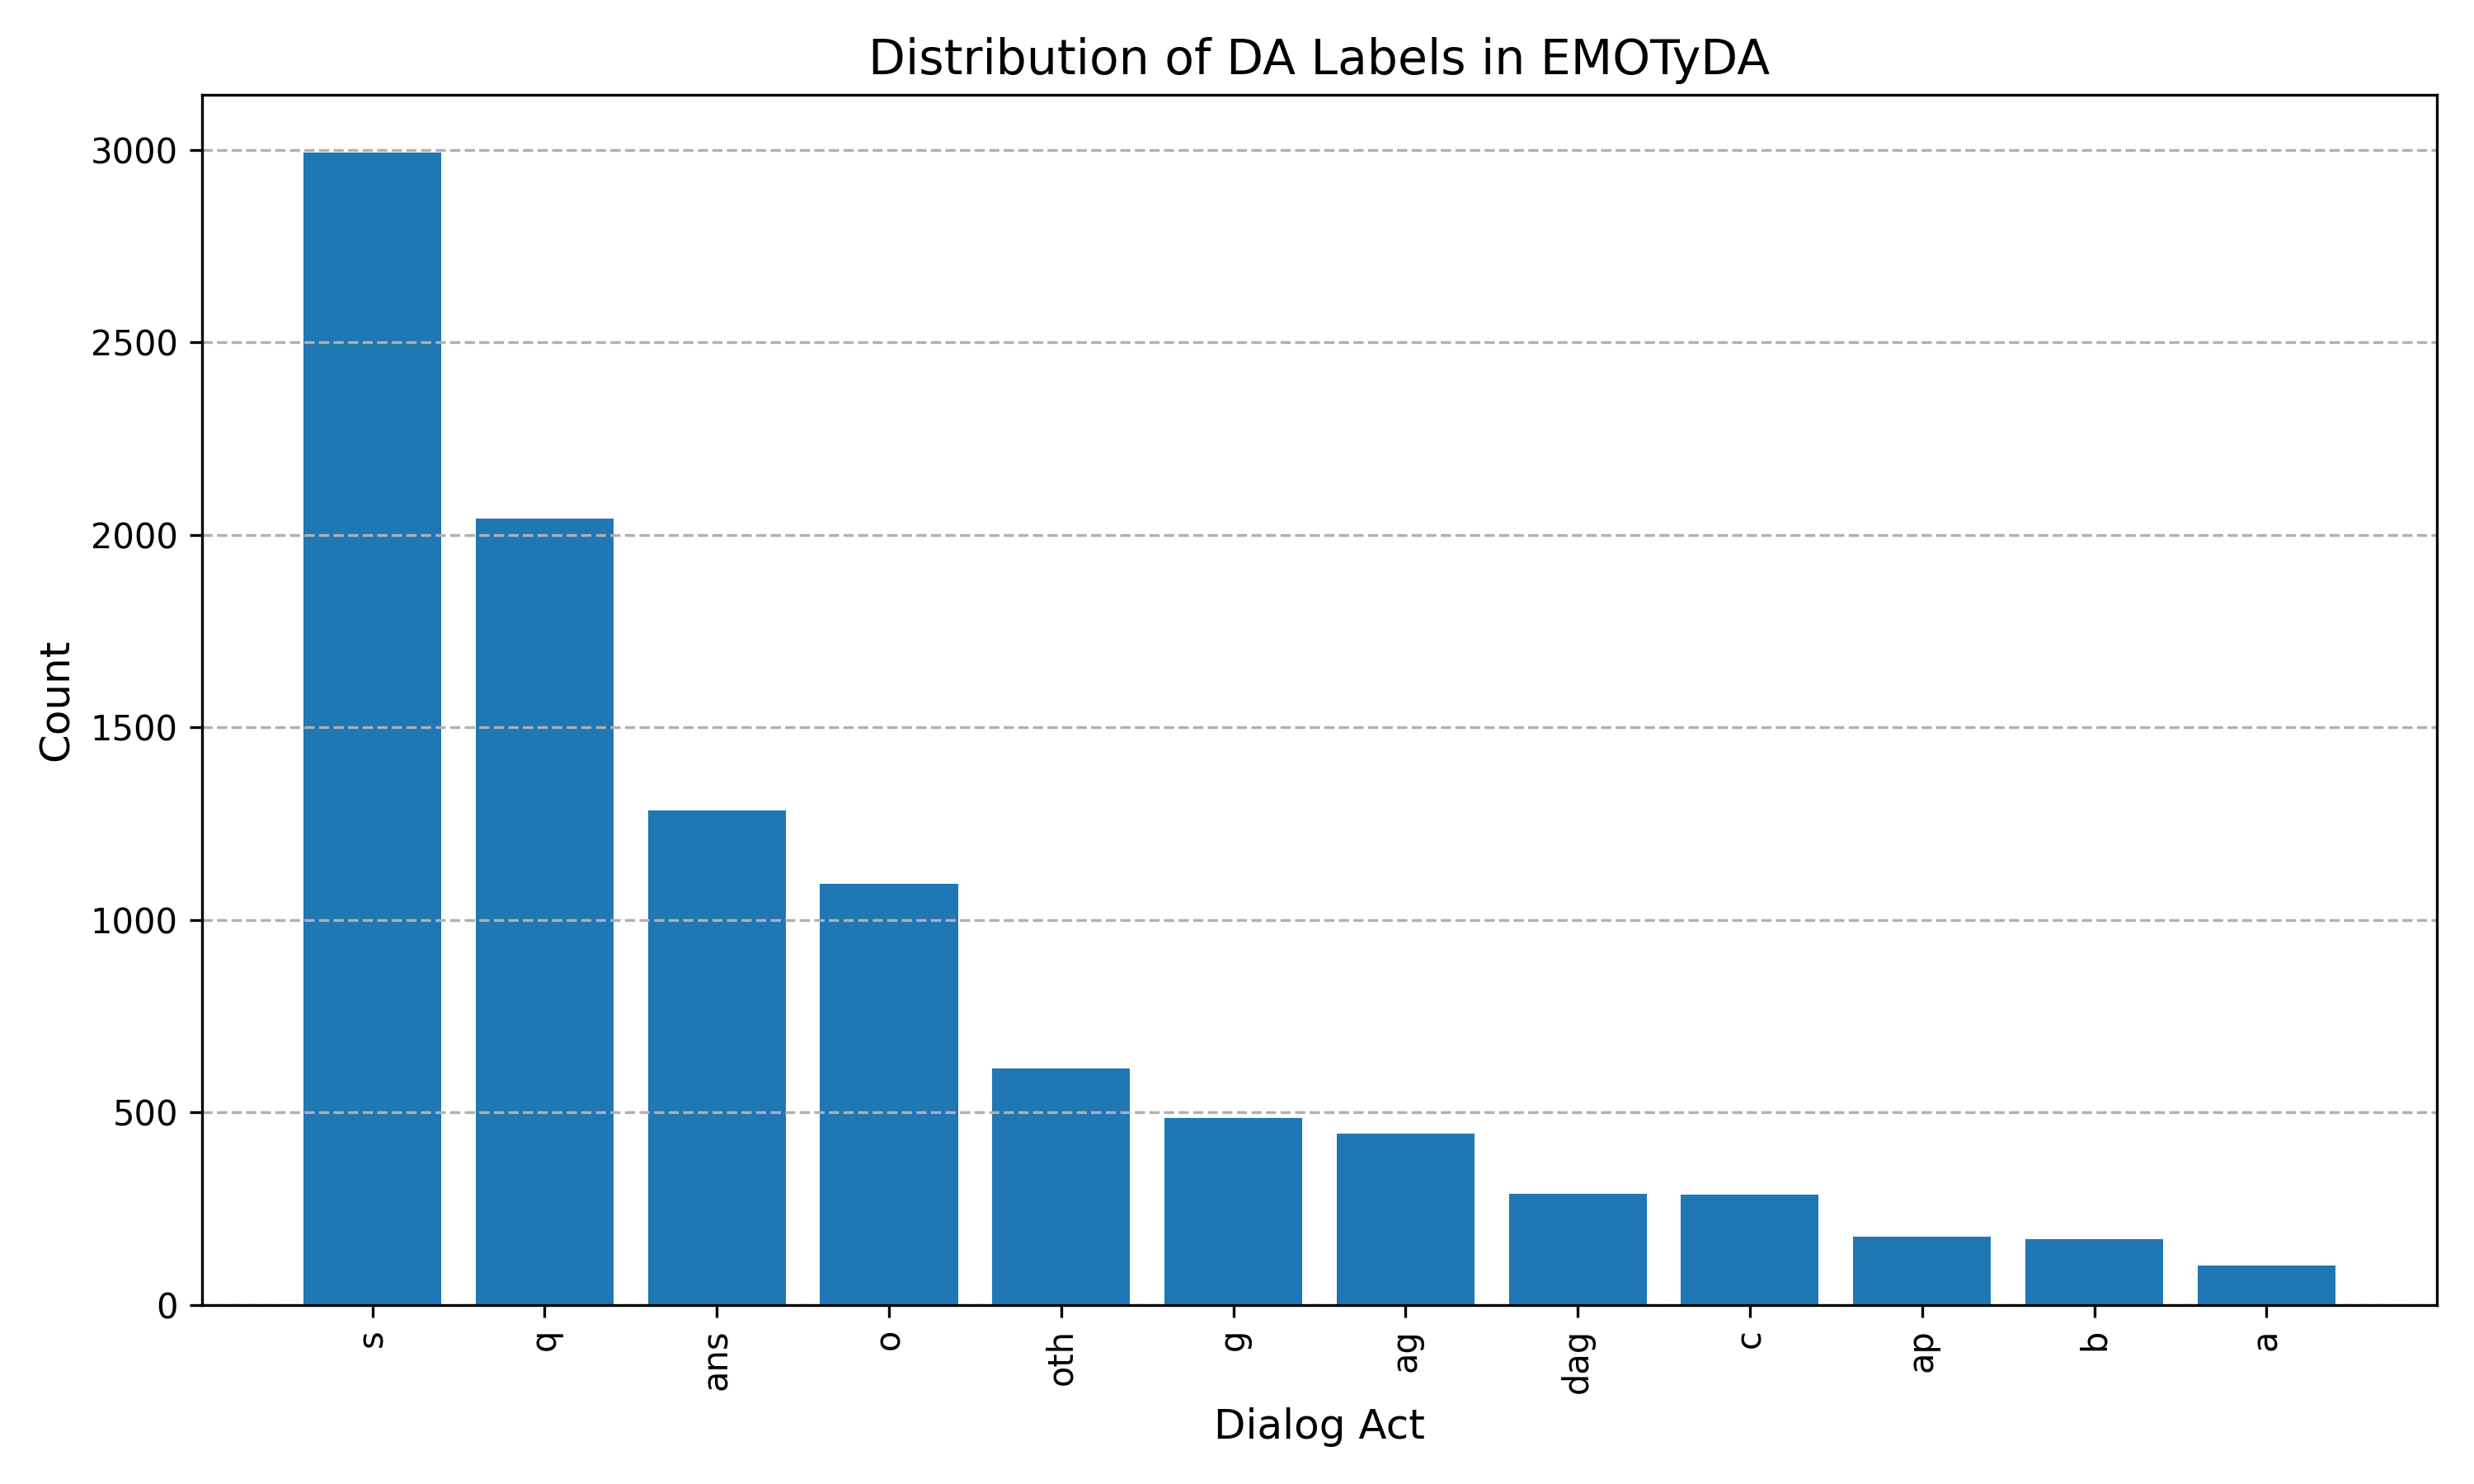
\includegraphics[width=\textwidth, scale = 5]{images/da_tag3_counts_EMOTYDA.png}
    \caption*{(b) EMOTyDA}
    \label{fig:image2}
  \end{minipage}
  \caption{Label distribution of the two datasets.}
  \label{fig:label_distribution}
\end{figure*}

\section{Configuration of Textual Feature Extraction}
\label{sec:roberta configuration}
We use pre-trained RoBERTa as feature extractor to extract token embeddings from the textual input. The choice of this feature extractor is consistent with contemporary works on DA classification \cite{he-etal-2021-speaker-turn} and other NLP tasks \cite{zheng-etal-2023-facial, chudasama2022m2fnet} in the literature. RoBERTa is also more recent and proven to be better than BERT on several NLP benchmarks and hence a better choice of feature extractor. 

We experimented with two variants of RoBERTa features, one where the token embeddings are the average of last 4 hidden states and the other where the token embeddings are solely from last hidden state. As shown in \autoref{tab:roberta}, we did not find any significant improvement using the intermediate layers and hence continued with the last hidden states for feature extraction for all the experimentation.

\begin{table}
  \centering
  \small
  \begin{tabularx}{\linewidth}{Xlc}
    \toprule
    Feature & Macro F1 & Accuracy \\
    \midrule
    Last hidden state & \textbf{29.11} & \textbf{59.86} \\
    Average of last 4 hidden states & 28.42 & 59.34  \\
    \bottomrule
  \end{tabularx}
  \caption{Comparison of different configurations of RoBERTa features}
  \label{tab:roberta}
\end{table}


\section{Configuration of Audio Feature Extraction}
\label{sec:whisper configuration}
For extracting frame embeddings from the audio, we used the pre-trained model, Whisper and followed the same setup that is used in original Whisper implementation for pre-processing audio inputs. The input audio utterance is padded or clipped to 30s and a 25ms window with 10 ms stride is employed to extract the mel-spectrograms. The choice of window size and stride for Whisper is consistent with that of other audio feature extraction methods across the literature. The final output from the whisper encoder is 1500 frames per utterance with 512 dimensional embedding per frame. 

\section{Hyperparameters}
\label{sec:hyperparameters}

To control the learning rate, we implemented a linear LR scheduler that gradually decreased the rate from the initial value of 1e-3 after 5 epochs.
For the MRDA dataset, our experiments are conducted over 40 epochs, while for the EMOTyDA dataset, the experiments were carried out for 20 epochs. To prevent overfitting, we used early stopping, ceasing training if no improvement in validation macro F1 score was observed for 5 consecutive epochs.  

The best model for inference on the test set was selected based on macro F1 score on the validation set.
To ensure the reliability of the results, each experiment was repeated 5 times with different random seeds, and the reported results represent the average performance across these runs.

A list of hyperparameters and the chosen values upon experimentation is shown in \autoref{tab:hyperparameters}.

\

\begin{table}
  \centering
  \small
  \begin{tabularx}{\linewidth}{Xc}
    \toprule
    Name & Best Value\\
    \midrule
    Hidden dimensions of encoders & 128\\ 
    Kernel size & 5\\
    No of channels for conv layers & 256\\
    Window size for context modeling & 3\\
    \bottomrule
  \end{tabularx}
  \caption{Choice of hyperparameters}
  \label{tab:hyperparameters}
\end{table}




\section{Training and Inference}
\label{sec:model_training}
All experiments were performed on a single NVIDIA RTX A6000 GPU.
Training an epoch on the MRDA dataset took approximately 40 minutes, with an additional 12 minutes each for validation and testing. Training time can be reduced by caching the audio features but it in turns increase the memory requirement on the CPU. Training an epoch on the EMOTyDA dataset took approximately 7 minutes, with an additional 2 minutes each for validation and testing. The latency of the model at inference time is 0.16 seconds to infer dialog act for each utterance.